
\section{SQL}

\begin{frame}[fragile,allowframebreaks]{Structured Query Language (SQL)}
  \metroset{block=fill}
\begin{block}{Database functions}
\begin{itemize}
    \item \textbf{SQL:} \emph{standardized} query language for relational databases
    \item \textbf{Data Definition Language (DDL):} create database
    \item \textbf{Data Manipulation Language (DML):} query and modify data 
    \item \textbf{Data Storage Description Language (DSDL):} write data on physical storage structure
\end{itemize}
\end{block}

\begin{exampleblock}{Ressources/Tutorials}
\begin{itemize}\footnotesize
    \item  \textbf{SQL:} \protect\url{ https://www.w3schools.com/sql/ }
    \item  \textbf{SQLite:} \protect\url{https://www.sqlitetutorial.net }
    \item \protect\url{https://sqlite.org/cli.html}
\end{itemize}
\end{exampleblock}


\begin{alertblock}{Good to know}
\mycommand{*}{sog. \emph{Wildcard}, matches/means: everything}
\mycommand{;}{expected as an end marker for SQL statements (not just ENTER)}
\end{alertblock}


\begin{alertblock}{\texttt{.dot} commands versus \texttt{;}}
\footnotesize
Using \texttt{.} tells the software to use an internal command from a fixed set of commands and not wait for \texttt{;} $\to$ only works for this predetermined set of commands!
\end{alertblock}

\begin{alertblock}{Open SQLite-shell (SQL commands)}
\mycommand{.shell cd directory }{change directory}
\mycommand{.save dbname }{save database}
\mycommand{.open dbname }{open previously saved db}
\end{alertblock}

\begin{exampleblock}{Using SQL}
\begin{enumerate}
    \item via the \alert{Terminal} (=commandline); in Windows \texttt{cmd} (search for it) $\to$ click \texttt{sqlite3.exe} or type \texttt{sqlite3}: 
    \begin{itemize}
        \item if there is no error, it's working and waiting for prompts!
        \item more info on SQLite CLI: \protect\url{https://sqlite.org/cli.html}
    \end{itemize}
    \item via \alert{SQLiteBrowser} (not recommended)
    \item possible \alert{file endings} to import: \texttt{.csv}, \texttt{.db}, \texttt{.sql}
\end{enumerate}
\end{exampleblock}


\begin{alertblock}{Special commands to sqlite3 (dot commands)}
 \mycommand{.help}{overview over dot commands}
\mycommand{.open ?OPTIONS? ?FILE? }{open or create db}
\mycommand{.databases }{show existing dbs}
\mycommand{.tables ?TABLE? }{show existing tables}
\mycommand{.import FILE TABLE }{import data to table}
\mycommand{.mode MODE ?TABLE? }{how to display output}
\mycommand{.mode column}{show \texttt{SELECT} results as tabular format}
\mycommand{.headers on}{show \texttt{SELECT} results with headers}
\mycommand{.schema ?TABLE? }{displays \texttt{CREATE} command used}
\mycommand{.save ?FILE? }{save the db}
\mycommand{.dump ?TABLE?}{show database contents as SQL commands}
\end{alertblock}

\end{frame}


%------------------------------------------------------------------------------
\begin{frame}[fragile]{Tutorial: Beginner SQL using SQLiteBrowser or Terminal}
\small
%oder einfach:
\begin{verbatim}
    > sqlite3 studis.db
\end{verbatim}
 
\begin{columns}
\column{0.45\textwidth}
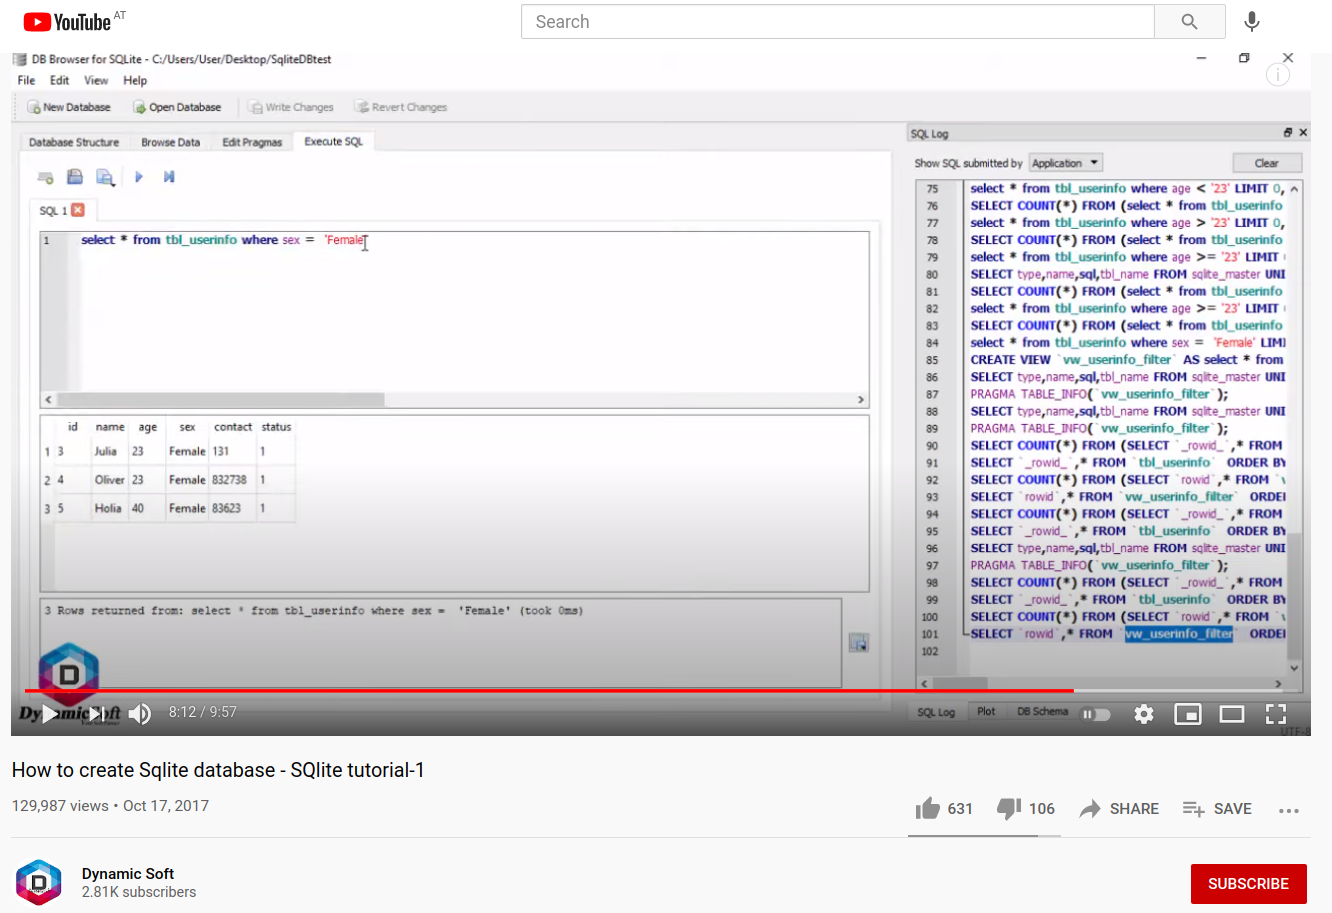
\includegraphics[width=0.8\textwidth]{img/youtube-sqlitebrowser.png}

ca. 10min Video \\
\protect\url{https://www.youtube.com/watch?v=Pni6WxHFTUg} \\

\column{0.45\textwidth}
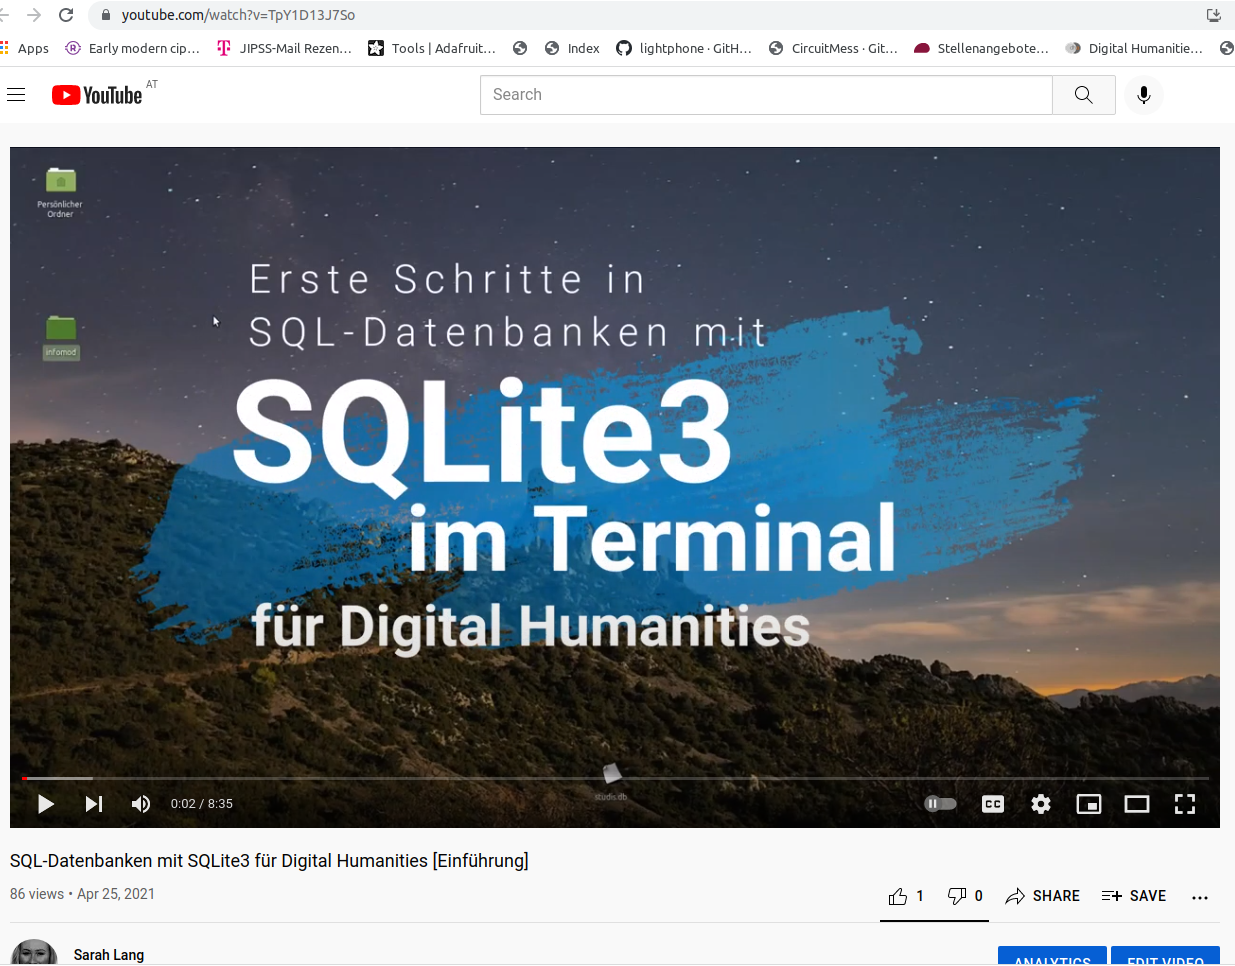
\includegraphics[width=0.8\textwidth]{img/sql-basics-video-youtube.png}

ca. 8min \\
\protect\url{https://www.youtube.com/watch?v=TpY1D13J7So&t=413s} \\

\end{columns}
\end{frame}


%------------------------------------------------------------------------------
\begin{frame}[fragile]{Some more SQL}
  \metroset{block=fill}
  \begin{columns}[T,onlytextwidth]
    \column{0.4\textwidth}
    
      \begin{block}{selection criteria}
        \begin{itemize}\footnotesize
            \item %Testausdruck: Feldname Operator Wert; Operator kann sein z.B. 
            Use operators like \texttt{=, !=, >, <, LIKE, REGEX, MATCH, ISNULL, NOTNULL}
            \item %Verknüpfung von mehreren Testausdrücken mit 
            Combine using \texttt{AND} or \texttt{OR}
        \end{itemize}
      \end{block}
      
    \column{0.55\textwidth}
\begin{block}{Print results}
\begin{sqlcode}
SELECT content 
FROM Tabelle 
WHERE selectionCriteriaMatch
\end{sqlcode}
\end{block}

\begin{block}{Reduce set of results}
  \begin{sqlcode}
SELECT content 
FROM Tabelle 
WHERE selectionCriteriaMatch
LIMIT max number of results
OFFSET results starting from...
\end{sqlcode}
\end{block}

  \end{columns}
\end{frame}


%------------------------------------------------------------------------------
\begin{frame}[fragile]{Delete or modify tables (DDL)}

\begin{block}{Delete table }
  \begin{sqlcode}
  DROP TABLE tableName;
  \end{sqlcode}
\end{block}

\begin{block}{Rename table }
  \begin{sqlcode}
  ALTER TABLE tableName RENAME TO tableName;
  \end{sqlcode}
\end{block}

\begin{block}{Add column}
  \begin{sqlcode}
  ALTER TABLE tableName 
  ADD COLUMN columnname1 datatype options;
  \end{sqlcode}
\end{block}
\end{frame}

%------------------------------------------------------------------------------
\begin{frame}[fragile]{Insert data = data representation (DML)}

\begin{block}{Add new row}
  \begin{sqlcode}
INSERT INTO tableName 
       (columnname1, columnname2, columnname3 [etc.]) 
       VALUES (value1, value2, value3 [etc.]);
\end{sqlcode}
\end{block}

\begin{block}{add multiple rows at a time}
  \begin{sqlcode}
VALUES (value1, value2, value3 [etc.]), 
       (value1, value2, value3 [etc.]), 
       (value1, value2, value3 [etc.]) [etc.]; 
\end{sqlcode}
\end{block}

\end{frame}


%------------------------------------------------------------------------------
\begin{frame}[fragile, allowframebreaks]{Example: delete or change entries (DML) }
\begin{block}{Change entries}
    \begin{sqlcode}
UPDATE tableName 
SET columnname_to_modify = new_value
WHERE columnname = referenceValue;
\end{sqlcode}
\end{block}

\begin{block}{Delete entries}
  \begin{sqlcode}
DELETE FROM tableName 
WHERE columnname = value;
\end{sqlcode}
\end{block}

\framebreak

\begin{block}{Query the db (DML) }
  \begin{sqlcode}
SELECT * FROM tableName;
SELECT table1, table3 FROM tableName;
\end{sqlcode}
\end{block}

\framebreak

German video slowly showing all steps from the first basic example: 

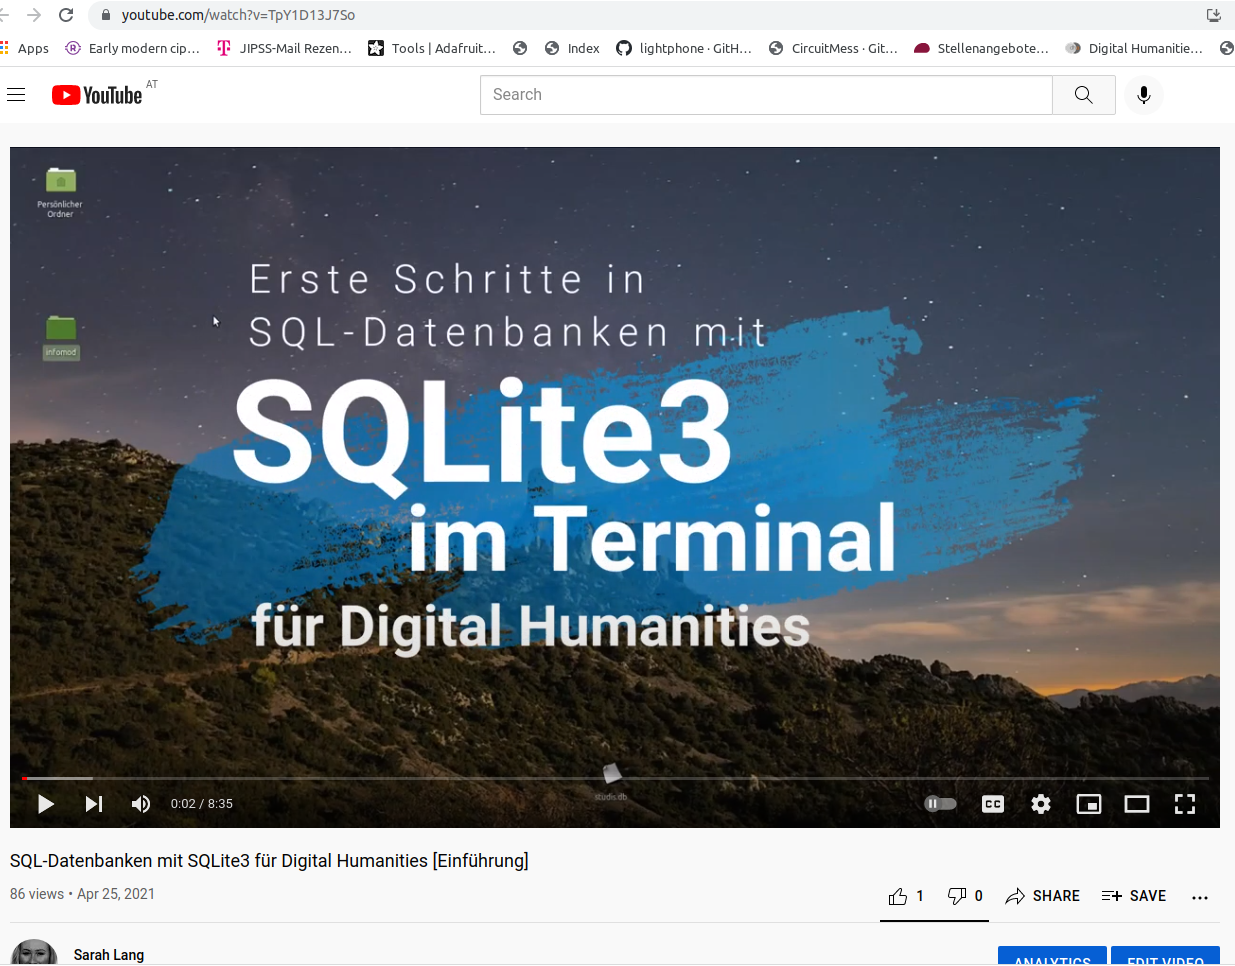
\includegraphics[width=0.65\textwidth]{img/sql-basics-video-youtube.png}

\framebreak

Our example from the intro.

\begin{columns}
\column{0.42\textwidth}
\begin{sqlcode}
.tables

ALTER TABLE studis
ADD COLUMN fachgebiet_id INT;

CREATE TABLE fachgebiet (
name TEXT,
id INT PRIMARY KEY
);

.tables
\end{sqlcode}

\column{0.58\textwidth}
\begin{sqlcode}
INSERT INTO fachgebiet (name, id)
VALUES ('dh', 1), ('geschichte', 2);

UPDATE studis 
SET fachgebiet = 2
WHERE id = 1;

SELECT * FROM studis;

SELECT name, fachgebiet 
FROM studis;
\end{sqlcode}
\end{columns}

\end{frame}

% Erstellen Sie mind. eine Entitätenmenge oder Beziehungsmenge (Tabelle) Ihres Originals mithilfe von SQL in der Kommandozeile. Laden Sie die Datenbank (.db) auf Moodle hoch.


%------------------------------------------------------------------------------
\begin{frame}[standout]
    What can you do with \alert{\texttt{urlaub.db}}?
\end{frame}

%------------------------------------------------------------------------------
\begin{frame}[standout]
    \alert{Homework 4: } Get started creating your database! \\[0.5em]
    \small Create a project database for your final project in SQL. 
    Write 1/2-1 page of text (submitted as PDF) explaining the following questions:
    {\footnotesize 
    \begin{itemize}
        \item  Which original are you modelling?
        \item What is the purpose of the database? Which queries do you want to answer with it?
        \item Which entities of the original are represented in your database?
        \item Which attributes (incl. Primary Keys) do the classes have?
\end{itemize}
    }
    Also submit a dump of your database please.
\end{frame}

%------------------------------------------------------------------------------
\begin{frame}[fragile]{SQL basics}
\begin{columns}
  \column{0.6\textwidth}
  \begin{enumerate}\footnotesize
      \item Our terminal expects that all statements are terminated by \texttt{;} -- this allows you to use line breaks to structure your query for better overview. If you forget the semicolon the terminal will keep waiting for input. It might look like it's stuck: Just type semicolon plus enter to fix it. 
      \item Asterisk (\texttt{*}) is a so-called \emph{wildcard} and means `everything'.
      \item Our simple first statement thus means: `Select \emph{everything} from the table named \emph{table}.'
      \item You can open databases (\texttt{.db} or \texttt{.sql}) using \texttt{sqlite3 databasename.db} from the terminal.
  \end{enumerate}
  \column{0.35\textwidth}
    \metroset{block=fill}
    \begin{block}{My first SQL statement}
    \footnotesize
    Before running your first command, you might need to use the \texttt{.tables} command in \texttt{sqlite3} to learn which tables even exist in your database and/or how they are named  (dot-prefixed commands exceptionally need no semicolon to end them, just enter).
    \begin{sqlcode}
    SELECT * FROM table;
    \end{sqlcode}
\end{block}

\end{columns}
\end{frame}


%------------------------------------------------------------------------------
\begin{frame}[fragile]{SQL basics 2}
\begin{columns}
  \column{0.6\textwidth}
  \begin{enumerate}\footnotesize
      \item If there was a mistake in your command, you get an error message. If there is none we assume all is good and whatever you prompted the program to do actually happened. There might just not be a success message. But what you prompted the program to do might not have been exactly what you had \emph{intended} it to do, so inspect the results by displaying your database anew!
      \item After you change a database, check its contents using  \texttt{SELECT * FROM table;} $\to$ make sure the change effected was the one intended.
      \item By convention, SQL keywords are capitalized in AllCaps style to make them easily identifiable visually. This makes your code more readable but the program would also work with lowercase commands.
  \end{enumerate}
  \column{0.45\textwidth}
More complex example:
  \begin{sqlcode}
SELECT DISTINCT column_list
FROM table_list
JOIN table ON join_condition
WHERE row_filter
ORDER BY column
LIMIT count OFFSET offset
GROUP BY column
HAVING group_filter;
\end{sqlcode}
\end{columns}
\end{frame}


%------------------------------------------------------------------------------
\begin{frame}[fragile, allowframebreaks]{SQL SELECT}
\begin{sqlcode}
SELECT list_of_columns FROM list_of_tables;
\end{sqlcode}
\begin{exampleblock}{What the options mean\dots}
\begin{description}\footnotesize
  \item[list\_of\_columns] you can select multiple columns separated by comma or use asterisk (\texttt{*}) to select all
  \item[list\_of\_tables] defines which tables to select from. 
  \item[AS (alias)] allows you to name the column header for the output table
  \item[DISTINCT] only prints each unique value once; \textbf{usage:} \texttt{SELECT DISTINCT}
\end{description}
\end{exampleblock}

\framebreak
\small 
To select specific columns from multiple tables which share common column names, specify as follows:
\begin{sqlcode}
SELECT hotels.name, places.name FROM hotels, places;
\end{sqlcode}
For more clarity, give them more meaningful headers:
\begin{sqlcode}
SELECT hotels.name AS hotel_name, 
       places.name AS place_name 
FROM hotels, places;
\end{sqlcode}
Not specifying from which table will either print a cartesian product or produce an error like so:
\begin{sqlcode}
SELECT name FROM hotel, place;
-- Error: ambiguous column name: name
\end{sqlcode}
  %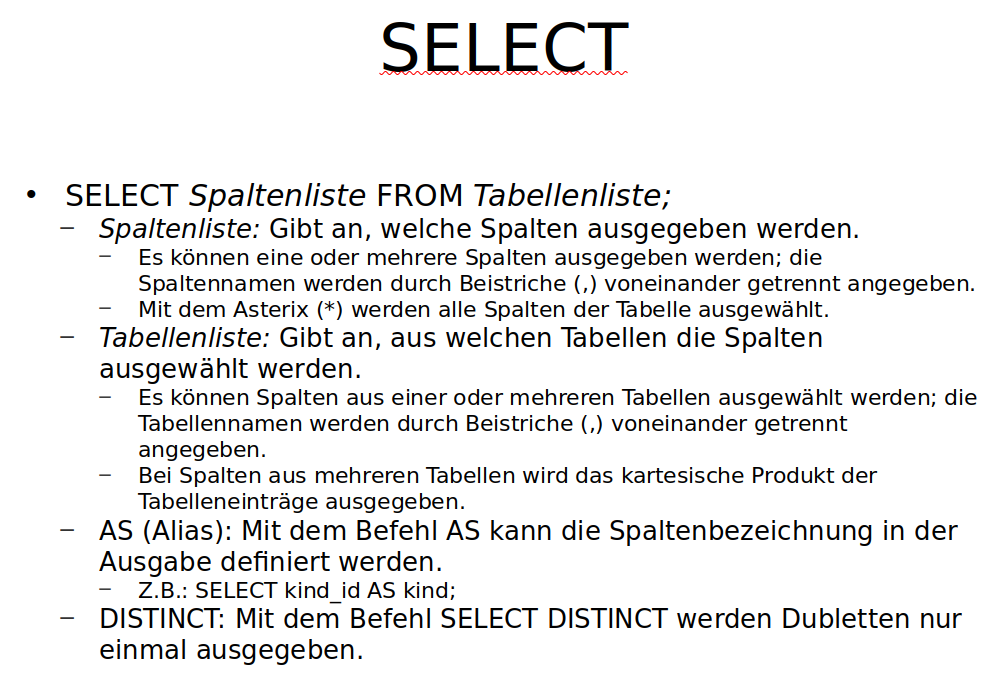
\includegraphics[width=\textwidth]{img/select-ueberblick.png} 

\end{frame}


%------------------------------------------------------------------------------
\begin{frame}[fragile]{SQL WHERE}
\small 
Entries are selected depending on the values of their attributes which are communicated using the following operators:
\begin{columns}
  \column{0.33\textwidth}
  \begin{block}{Comparison operators}
    \begin{description}\footnotesize
      \item[=] equals
      \item[>] greater than
      \item[<] less than
      \item[>=] greater or equal
      \item[<=] less or equal
      \item[!= or <>] not equal
    \end{description}
  \end{block}

  \column{0.66\textwidth}
  \begin{block}{Logical operators}\footnotesize
    \begin{description}
      \item[AND] both are true
      \item[OR] at least one part is true
      \item[BETWEEN] value is within a defined range
      \item[IN] value in included in defined set
      \item[LIKE] value corresponds to a pattern
      \begin{description}
        \item[\%] any sequence of characters (none or multiple)
        \item[\_] any one character (exactly one)
      \end{description}
      \item[NOT] results in the opposite of the truth value of the expression
    \end{description}
  \end{block}
\end{columns}
\begin{sqlcode}
SELECT name FROM hotel WHERE price < 150;
\end{sqlcode}
  %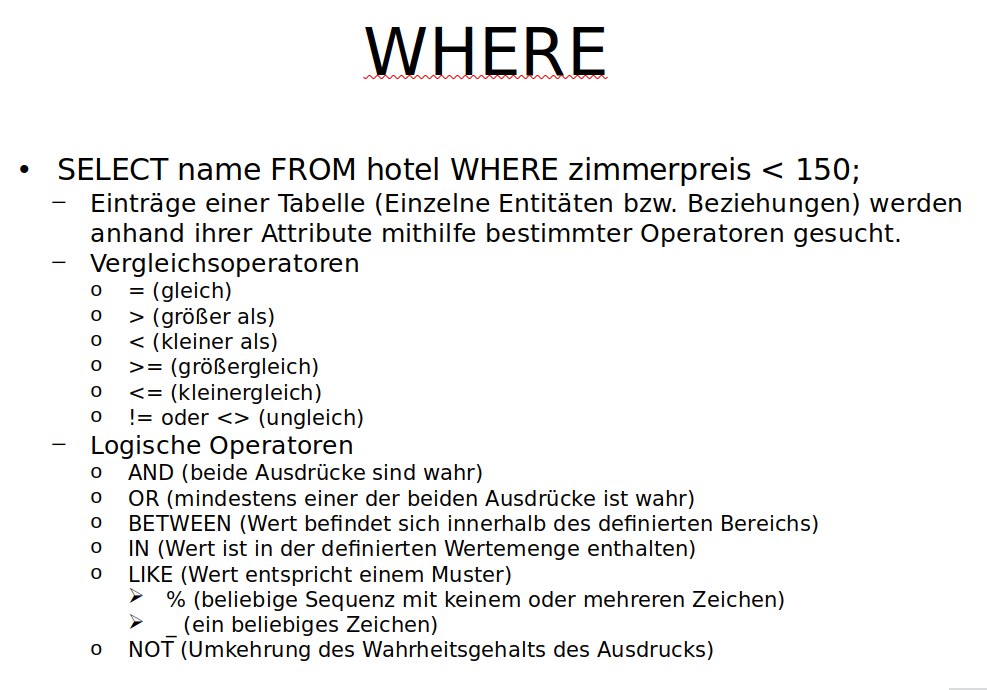
\includegraphics[width=\textwidth]{img/sql-where.png}  
\end{frame}

%------------------------------------------------------------------------------
\begin{frame}[fragile, allowframebreaks]{SQL CREATE VIEW}

  If you need to rearrange the order of your table after it is already defined or just getting an output that you often need is very complicated and annoying, you might want to create a \texttt{VIEW} so that you can access the result of a complex query over and over again effortlessly:
  \begin{sqlcode}
CREATE VIEW view_name AS
SELECT column1, column2, ...
FROM table_name
WHERE condition; 
  \end{sqlcode}
  It will always show up-to-date data as it's just a shorthand for the actual complex query. 
  \framebreak
  
  \href{https://www.w3schools.com/sql/sql_view.asp}{W3C Tutorial 'CREATE VIEW'} $\to$ \textbf{examples:}
        \begin{sqlcode}
CREATE VIEW [Brazil Customers] AS
SELECT CustomerName, ContactName
FROM Customers
WHERE Country = 'Brazil';

-- display as:
SELECT * FROM [Brazil Customers]; 
  \end{sqlcode}

        \begin{sqlcode}
CREATE VIEW [Products Above Average Price] AS
SELECT ProductName, Price
FROM Products
WHERE Price > (SELECT AVG(Price) FROM Products); 
-- call as:
SELECT * FROM [Products Above Average Price]; 
  \end{sqlcode}


\end{frame}


%------------------------------------------------------------------------------
\begin{frame}[fragile]{Creating tables (DDL)}
\begin{sqlcode}
CREATE TABLE tableName (
  columnName1 datatype option,
  columnName2 datatype option,
  [...]
  );
\end{sqlcode}
\begin{exampleblock}{What the options mean\dots}
\begin{description}\footnotesize
  \item[tableName] represents the entity set, written in lowercase.
  \item[columnName] represents an attribute or relationship of the entity, in lowercase. 
  \item[datatype] sets the data type from a list of possibilities such as \texttt{TEXT} or \texttt{INTEGER}, etc.
  \item[options] 
  \begin{itemize}
      \item \textbf{Primary Key:} \texttt{PRIMARY KEY} $\to$ sets value as primary key.
      \item \textbf{Foreign Key:} \texttt{FOREIGN KEY columnName REFERENCES tableName\_pk(attribute\_pk)} $\to$ sets value as foreign key.
      \item \textbf{No empty values allowed:} \texttt{NOT NULL}.
      \item \textbf{Values have to be unique:} \texttt{UNIQUE}.
  \end{itemize}
\end{description}
\end{exampleblock}
 % 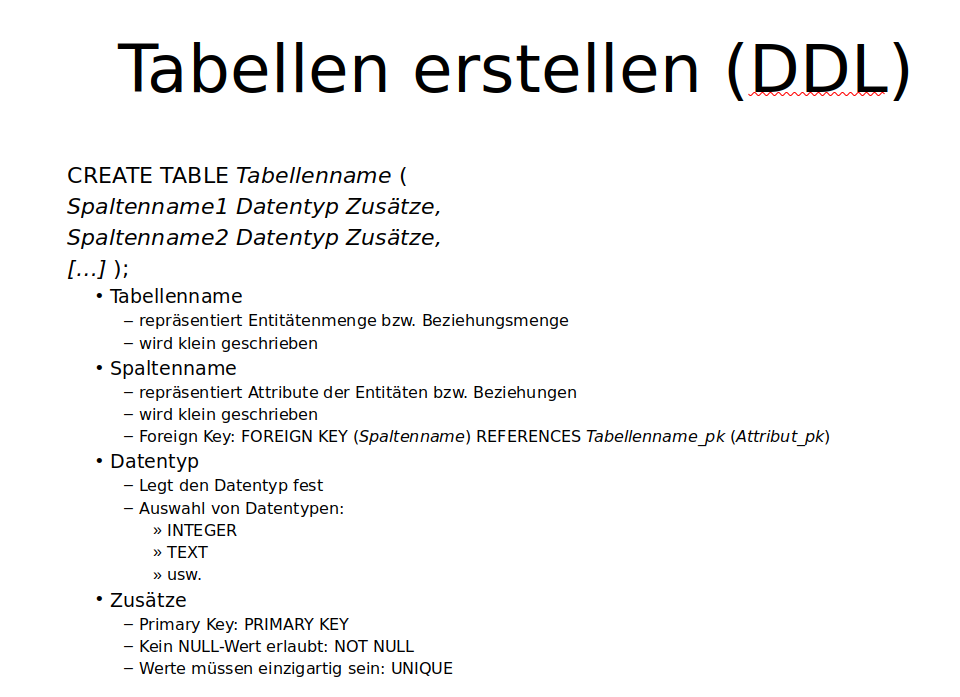
\includegraphics[width=\textwidth]{img/tabellen-erstellen-ddl.png}
\end{frame}



%------------------------------------------------------------------------------

\section{Database organization, Primary and Foreign Keys}
%------------------------------------------------------------------------------
\begin{frame}[fragile]{Data types}
  \metroset{block=fill}\footnotesize
      \begin{alertblock}{Data types}
        \begin{itemize}
            \item \textbf{NULL} nothing
            \item \textbf{INTEGER} positive integer values (Ganzzahlen)
            \item \textbf{REAL} 8-byte IEEE floating point values
            \item \textbf{TEXT} text encoded according to DB standard (UTF-8, UTF-16BE or UTF-16LE).
            \item \textbf{BLOB} The value is a blob of data, stored exactly as it was input.
        \end{itemize}
      \end{alertblock}
      
      Other database management systems (DBMS) have a slightly different choice of datatypes due to different implementations. \textbf{Remember: }SQL is a standard which is implemented slightly differently by different software solutions such as \texttt{SQLite3} or \texttt{MySQL} (\alert{\href{https://www.w3schools.com/sql/sql_datatypes.asp}{check out this list}}).
      
      In MySQL, instead of \texttt{TEXT} you would use this:
      \begin{sqlcode}
          LastName varchar(255),
      \end{sqlcode}
      This tells the computer exactly for how many characters it needs to reserve space. This used to be more important especially when computer memory was more rare a commodity than it is today.  
      
\end{frame}


%------------



%------------------------------------------------------------------------------
\begin{frame}[allowframebreaks]{Primary and Foreign Keys}
    % ----------------------------------------------
{\scriptsize Source: Gunter Vasold, \emph{Datenbanken} class (summer term 2017)}
\metroset{block=fill}

      \begin{block}{}
      \centering 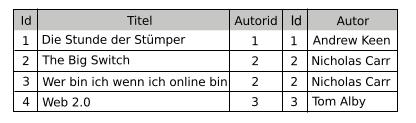
\includegraphics[width=0.48\textwidth]{img/autor-id-titel.png}~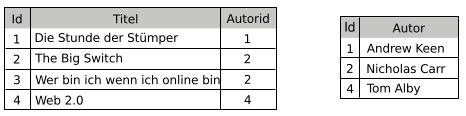
\includegraphics[width=0.48\textwidth]{img/foreign-key.png}
      \end{block}

\begin{itemize}\scriptsize
\item Because relations are sets, each tuple needs to be different from all others. To address one specific tuple, we need a key or an id. This key needs to be unique in the whole relationship set. 
\item A key (\emph{primary key}, \textbf{Primärschlüssel}) can consist of one or multiple attributes (as few as possible, it has to be irreducible or minimal). In practice, we often use artificial keys (like a running id number). 
\item \textbf{Foreign keys} (\emph{Fremdschlüssel}) reference the primary key of a tuple in a different relation. Because foreign keys don't need to be unique, they aren't technically keys but are still called that way. Comparing foreign and primary keys, we can create new relations ad hoc.
\end{itemize} 
    %\begin{block}{}\centering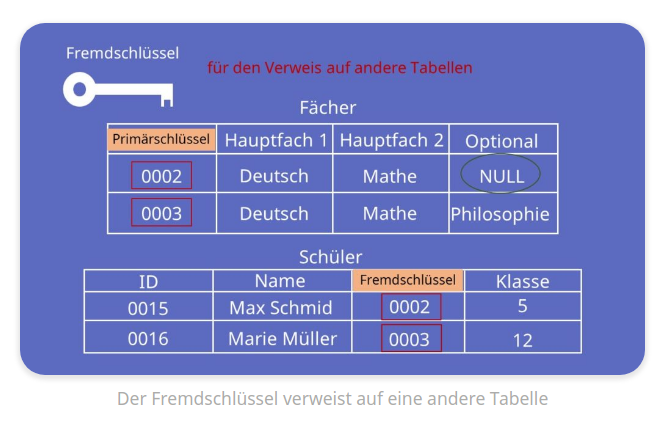
\includegraphics[width=0.9\textwidth]{img/foreign-keys-studyflix.png}\end{block} % https://studyflix.de/informatik/relationale-datenbanken-600

\framebreak

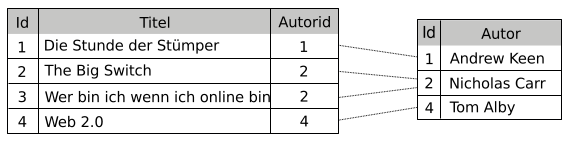
\includegraphics[width=0.9\textwidth]{img/foreign-keys-linked.png}\bigskip

\metroset{block=fill}  
      \begin{exampleblock}{Referential integrity}\footnotesize
Referential integrity is a constraint which ensures that a dataset can only be manipulated if it doesn't render other datasets inconsistent. 

\textbf{Example:} Deleting dataset with \texttt{id=4} in the table \texttt{author} would destroy referential integrity because at least one foreign key in the table \emph{book} references this entry. For the machine to automatically know that, we need to declare these keys and their relationships when setting up the database (more on that later).
      \end{exampleblock}
\end{frame}
%------------------------------------------------------------------------------
\begin{frame}[fragile, allowframebreaks]{Unique Identifiers: Primary and Foreign Keys}
  \metroset{block=fill}
\begin{exampleblock}{Identifier}
\textbf{unique identifier / key:} refers to exactly one element. Examples: \vspace{-1em}
      \begin{enumerate}
          \item ISBN no.
          \item matriculum nr.
          \item ORCID-ID
          \item DOI
          \item car plate
          \item norm data (GND): list of standardized terminoloy, gives a definite name form and an ID to refer to
      \end{enumerate}
      \end{exampleblock}
      
\begin{exampleblock}{Indirection} An ID doesn't directly point to a value but rather to a number which, in turn, points to the value. 
\end{exampleblock}

\begin{exampleblock}{Separating contents into multiple tables minimizes redundancy!}  
Data can be reunited (joined) using \texttt{VIEW}s. Redundancy is a source of errors.
\end{exampleblock}
\framebreak 

Each table needs to have its primary key. You can define it in the two following ways:
\begin{enumerate}\small 
    \item as an added option when defining the column:
\begin{sqlcode}
id INT PRIMARY KEY
\end{sqlcode}
    \item as an extra option after all column definitions:
\begin{sqlcode}
PRIMARY KEY(id)
PRIMARY KEY(forname, lastname, birthday)
\end{sqlcode}
\end{enumerate}

\begin{alertblock}{Resources}
  \begin{enumerate}\footnotesize
      \item \href{https://www.w3schools.com/sql/sql_primarykey.asp}{W3Schools Primary Key}: unique identifier for each table entry
      \item \href{https://www.w3schools.com/sql/sql_unique.asp}{W3Schools UNIQUE}
      \item \href{https://www.w3schools.com/sql/sql_notnull.asp}{W3Schools NOT NULL}
  \end{enumerate}
\end{alertblock}

\end{frame}

%------------------------------------------------------------------------------
\begin{frame}[fragile]{Linking tables}
  \metroset{block=fill}
  Example: Linking tables using keys \bigskip 
\small 
\begin{columns}
  \column{0.3\textwidth}
    \begin{block}{}
        \begin{enumerate}
            \item \textbf{Class:} \underline{ClassID}, LecturerID, subject, RoomID, hours
            \item \textbf{Room:} \underline{RoomID}, building, capacity
            \item \textbf{Lecturer:} \underline{LecturerID}, name, area of expertise
            \item \textbf{Student:} \underline{StudentID}, name, area of study
        \end{enumerate}
      \end{block}
  \column{0.72\textwidth}
Generic example:
\begin{sqlcode}
CREATE TABLE person (
   id      INTEGER PRIMARY KEY AUTOINCREMENT,
   name    TEXT   NOT NULL,
   age     INT    NOT NULL,
   address TEXT
);
\end{sqlcode}

Class example:
\begin{sqlcode}
CREATE TABLE student (
   student_id      INTEGER PRIMARY KEY,
   name            TEXT    NOT NULL,
   degreeProgramme TEXT    NOT NULL
);
\end{sqlcode}
\end{columns}
\end{frame}


%------------------------------------------------------------------------------
\begin{frame}[fragile, allowframebreaks]{Using Foreign Keys join tables}
\metroset{block=fill}
\footnotesize

Each table only contains one type of entity (e.g. student's names and ID numbers). But these might have relationships to other tables, for example, for each student we could list course numbers. Using this course number we get a link to a course table where we write down the name of the class.


\begin{alertblock}{Foreign Keys (\emph{Fremdschlüssel})}
\footnotesize
It is not mandatory to specify Foreign Keys but they allow the database to run internal optimization in the background. They are essential for maintaining referential integrity. 

You can define them as follows:
\begin{enumerate}
    \item as part of the respective column definition:
\begin{sqlcode}
REFERENCES tableNname(fieldName)
\end{sqlcode}
    \item after the column definitions:
\begin{sqlcode}
FOREIGN KEY(columnName) REFERENCES tablenName(fieldName)
\end{sqlcode}
\end{enumerate}
\end{alertblock}

\framebreak 
Assuming there were another table called \texttt{places}
with the primary key \texttt{id}
\begin{sqlcode}
CREATE TABLE persons (
  place_id INT UNSIGNED REFERENCES places(id),
  ...
);

CREATE TABLE persons (
  place_id INT UNSIGNED ,
  ...
  FOREIGN KEY (place_id) REFERENCES places(id)
);
\end{sqlcode}
\framebreak 

This \emph{Foreign Key} refers to another table's \emph{Primary Key}. 
Assuming there is a \texttt{disciplineID} in the \texttt{disciplines} table where it is the\emph{Primary Key}. 
In the \texttt{Students} table would be a column called \texttt{disciplineID} which is a foreign key \emph{Foreign Key there.}


\begin{block}{Foreign Key constraints in \texttt{CREATE TABLE}}
\begin{sqlcode}
FOREIGN KEY (columnName) 
REFERENCES tableName_pk (attribute_pk)
PRAGMA foreign_keys = ON;
\end{sqlcode}
\end{block}

Using \texttt{FOREIGN KEY} constraints we could define what happens if, for example, one of the related tables gets updated or something is deleted. 
\end{frame}

%------------------------------------------------------------------------------
\begin{frame}[fragile, allowframebreaks]{Constraints}
\metroset{block=fill}
\footnotesize

\begin{alertblock}{\href{https://www.w3schools.com/sql/sql_constraints.asp}{W3Schools SQL Constraints}}
  \begin{description}\footnotesize 
      \item[NOT NULL] makes sure a field can never be \texttt{NULL} (important for IDs). 
      \item[UNIQUE] makes sure all values of a column are distinct (also important so that IDs remain unique). 
      \item[PRIMARY KEY] automatically creates a combination of \texttt{NOT NULL} and \texttt{UNIQUE}, making the primary key an ideal means of referencing a table entry. 
      \item[FOREIGN KEY] prevents relationships between tables from accidentally getting destroyed (by the deletion of a cell, for example, to which the cells of another table still refer).
      \item[CHECK] makes sure the values of a column correspond to certain constraints (such as age is in between 0-99 or similar). This prevents you from accidentally inserting nonsensical values into the table which could later corrupt any analyses you might want to use the database for. 
  \end{description}
\end{alertblock}


\begin{alertblock}{Value constraints}
  Many DBMSs allow you to define any allowed range for value for a given column. Syntax:
\begin{sqlcode}
CHECK ([ fieldname ] [ condition ])
\end{sqlcode}

Example
\begin{sqlcode}
CREATE TABLE teachers (
salary DECIMAL (4 ,2) ,
CHECK ( salary > 0)
)
...
CHECK (grade >0 AND grade <=5)
\end{sqlcode}
\end{alertblock}

\end{frame}





%------------------------------------------------------------------------------
\begin{frame}{Excursus: SQL Injection (definition)}
  \metroset{block=fill}

  \begin{columns}
    \column{0.48\textwidth}
\begin{alertblock}{\href{https://en.wikipedia.org/wiki/SQL_injection}{Wikipedia}}\footnotesize
SQL injection is a code injection technique used to attack data-driven applications, in which malicious SQL statements are inserted into an entry field for execution (e.g. to dump the database contents to the attacker).
\end{alertblock}
\bigskip

\begin{block}{related \texttt{xkcd} comic} 
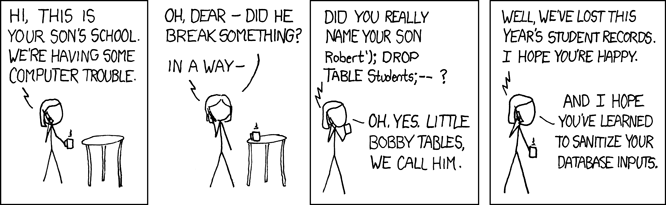
\includegraphics[width=0.95\textwidth]{img/exploits_of_a_mom.png}
\scriptsize
\href{https://xkcd.com/327/}{source}
\end{block}

\column{0.48\textwidth}
\begin{exampleblock}{\href{https://www.w3schools.com/sql/sql_injection.asp}{W3Schools}}\footnotesize
SQL injection is one of the most common web hacking techniques. 

SQL injection is the placement of malicious code in SQL statements, via web page input.

SQL injection usually occurs when you ask a user for input, like their username/userid, and instead of a name/id, the user gives you an SQL statement that you will \textbf{unknowingly} run on your database.
\end{exampleblock}
\end{columns}
\end{frame}

%------------------------------------------------------------------------------
\begin{frame}[fragile]{Excursus: SQL Injection (example from W3Schools)}
  \metroset{block=fill}

    \begin{block}{Starting point}
    \scriptsize
    A website gets data using a form to later run a database query whose results are to be displayed to the user. Example in javascript:
  \begin{jscode}
txtUserId = getRequestString("UserId");
txtSQL = "SELECT * FROM Users WHERE UserId ="
         + txtUserId;
  \end{jscode}
\end{block}

  \begin{columns}
    \column{0.48\textwidth}
\begin{block}{Always True Inject}\scriptsize
In case there are no security checks when parsing the submitted query, users can submit SQL code instead of just a normal value. 
\texttt{OR 1=1} is always true, thus all users will be displayed. Resulting SQL query (obviously it was not intended by the database owners to use the form like this):
  \begin{sqlcode}
  SELECT * FROM Users 
  WHERE UserId = 105 OR 1=1;
  \end{sqlcode}
\end{block}
\column{0.48\textwidth}
\begin{block}{Batched Statement Inject}\scriptsize
Instead of just running one statement, one could also add \texttt{;} and send a second query after it. For example by typing into the form: \texttt{105; DROP TABLE Users}. Resulting SQL code: 
  \begin{sqlcode}
  SELECT * FROM Users 
  WHERE UserId = 105; 
  DROP TABLE Users;
  \end{sqlcode}
\end{block}
  \end{columns}
\end{frame}



%------------------------------------------------------------------------------


\begin{frame}[fragile, allowframebreaks]{Cardinality}
\metroset{block=fill}

\begin{alertblock}{Cardinality}\small
Cardinality describes how many entities participate in a relationship. The following cardinalities are possible:
  \begin{description}\footnotesize
      \item[1:1] exactly one-to-one relationship, quite rare in practice.  \\\textbf{\scriptsize Example:} \emph{\scriptsize Student can only have one passport photo.}
      \item[1:n] (directionality can also be n:1 !) Exactly one entity is linked to one or multiple others.  \\\textbf{\scriptsize Example:} \emph{\scriptsize Student can have multiple adresses.}
      \item[n:m] Both parts of the relationship can participate in multiple relationships. \\\textbf{\scriptsize Example:} \emph{\scriptsize Students can go to multiple classes; most classes should have more than one student.}
  \end{description}
\end{alertblock}

\end{frame}

%------------------------------------------------------------------------------
\begin{frame}{Remember: How to represent entities in a database}
    \begin{itemize}
        \item \textbf{entity} $\to$ table
        \item \textbf{attribute} $\to$ column
        \begin{itemize}
            \item multi-valued attributed $\to$ helper table
        \end{itemize}
        \item \textbf{relationship}
            \begin{itemize}\footnotesize
                \item \textbf{1:1} $\to$ Key of one entity (table) is stored as reference (`foreign key'/`Fremdschlüssel') in the other table as a column/attribute of its own 
                \item \textbf{1:n} $\to$ key of the 1-ary entity/table stored as reference in the n-ary table/entity 
                \item \textbf{n:m} $\to$ table of its own containing the keys of both related entities
                \item \textbf{n-ary relations} $\to$ helper table containing the keys of all entities as columns 
                \item \textbf{relationship attributes} $\to$ helper table with the keys of participating entities and columns for the attributes 
                \item \textbf{multi-valued attributes} $\to$ helper table with entity key as foreign key (like a 1:n relation) and a column for the attribute 
                \item \textbf{composite attributes} $\to$ helper table with entity key as foreign key (like a 1:n relation) and columns for the partial attributes 
            \end{itemize}
    \end{itemize}
\end{frame}
  
\section{More advanced queries}
%------------------------------------------------------------------------------
\begin{frame}[fragile, allowframebreaks]{Functions, sorting, counting, etc.}
%\metroset{block=fill}

\begin{columns}
\column{0.44\textwidth}
\begin{block}{COUNT}
  \begin{sqlcode}
SELECT COUNT(columnname) 
FROM tablenname 
WHERE bedingung ;
\end{sqlcode}
\end{block}

\column{0.53\textwidth}
\begin{block}{AS}\small
Using \texttt{AS} you can rename columns in the output. \texttt{PricePerPage} would then be a derived attribute.\vspace{-1em}
\begin{sqlcode}
SELECT title AS Titel ,
price AS Price ,
price / pages AS PricePerPage
FROM books ;
\end{sqlcode}
\end{block}
\end{columns}

\framebreak

\begin{columns}
\column{0.47\textwidth}
\begin{block}{BETWEEN}\small
Only prints entries upon the condition that they are between two values:\vspace{-1em}
  \begin{sqlcode}
SELECT * FROM Products
WHERE Price BETWEEN 10 AND 20; 
\end{sqlcode}
\end{block}


\column{0.53\textwidth}
\begin{block}{DISTINCT}\small
Only prints distinct values (\emph{unique values}):\vspace{-1em}
  \begin{sqlcode}
SELECT DISTINCT columnname 
FROM table;

SELECT COUNT(DISTINCT columnname) 
FROM table;
\end{sqlcode}
\end{block}
\end{columns}


\framebreak 

\metroset{block=fill}


\begin{columns}
\column{0.47\textwidth}
\begin{block}{ORDER BY}\footnotesize
Sort the results of a query by one or multiple columns (separated by commata \texttt{,}) 
\begin{description}\scriptsize
\item[ASC] ascending order
\item[DESC] descending order
\end{description}
You can also sort by letters (e.g. alphabetically).

\begin{sqlcode}
ORDER BY fieldnames 
ORDER BY fieldname DESC 
SELECT name FROM hotel 
ORDER BY price ASC;
\end{sqlcode}
\end{block}

\column{0.47\textwidth}
\begin{block}{GROUP BY}\footnotesize
Lists each value as a row of its own:
  \begin{sqlcode}
SELECT AVG(columnnameX) 
FROM tablenname 
GROUP BY columnnameY;

SELECT rating, AVG(price)
FROM hotel 
GROUP BY rating;
\end{sqlcode}
\end{block}
\end{columns}

\framebreak

\begin{block}{Aggregate functions}\footnotesize
Functions offered by the database management system which aggregate data: They don't output single database entries but the result of a function the system calculated, e.g. \texttt{COUNT()}, \textbf{SUM()}, \texttt{MIN()}, \texttt{MAX()} and \texttt{AVG()}.
\end{block}
\bigskip

\begin{columns}
\column{0.53\textwidth}
\begin{block}{}\footnotesize % Funktionen für Zahlenwerte
$\to$ data fields with number values can be aggregated using:

\mycommand{AVG()}{average}
\mycommand{SUM()}{sum}
\mycommand{MIN()}{minimum value}
\mycommand{MAX()}{maximum value}

\end{block}
\column{0.38\textwidth}
  \begin{sqlcode}
SELECT MIN(column_name)
FROM table_name
WHERE condition;
\end{sqlcode}

\end{columns}

There are many more functions, operators, etc. than can be presented in the limited time here. 

\framebreak 

\footnotesize
Instead of \texttt{=} you can use the \texttt{LIKE} operator which allows for the use of wildcards (placeholders). 

\begin{columns}\footnotesize
\column{0.49\textwidth}
\begin{block}{Wildcard \texttt{\%} and \texttt{LIKE}}
Very powerful, in SQL use \texttt{\%} which stands of any characters (0-n).
\begin{sqlcode}
SELECT title
FROM books
WHERE title LIKE 'Datenbank %';

SELECT title
FROM books
WHERE title LIKE '% Datenbank';
\end{sqlcode}
\end{block}

\column{0.49\textwidth}
\begin{block}{Wildcard \texttt{\_} and \texttt{LIKE}}
\texttt{\_} = exactly one character.

\begin{sqlcode}
SELECT firstname, lastname
FROM authors
WHERE firstname LIKE 'g_nter';
\end{sqlcode}

Select all three-letter fornames:
\begin{sqlcode}
SELECT firstname
FROM authors
WHERE firstname LIKE '___';
\end{sqlcode}
\end{block}
\end{columns}

\begin{columns}\footnotesize
\column{0.47\textwidth}
\begin{block}{Special comparison operators: \texttt{IN} and \texttt{NOT IN}}
\footnotesize

\texttt{IN} compares against a list of values:

\begin{sqlcode}
SELECT title, year
FROM books
WHERE year IN (2000, 2004)
ORDER BY year;
\end{sqlcode}

\texttt{NOT IN} gives you the opposite of the set for which the condition is true:
\begin{sqlcode}
SELECT title, year
FROM books
WHERE year NOT IN (2000, 2008)
ORDER BY year;
\end{sqlcode}
\end{block}

\column{0.56\textwidth}
\begin{block}{Combining conditions with \texttt{AND}} 
\begin{sqlcode}
SELECT title, pages, price
FROM books
WHERE pages > 500 AND price < 10;
\end{sqlcode}
{\scriptsize
gives you all books which have more than 500 pages and whose price is still below 10€.

Combine as needed with other operators such as\texttt{OR} and \texttt{AND NOT}. 
If queries get very complicated, make sure to introduce clarity by the use of parentheses.

Here are books appeared after 2012 which are more than 500 pages long \emph{or} cost more than 30€:
}
\begin{sqlcode}
SELECT title , year , pages , price
FROM books
WHERE year > 2012 
AND (pages > 500 OR price > 30) ;
\end{sqlcode}
\end{block}
\end{columns}

\begin{columns}
\column{0.48\textwidth}
\begin{block}{LIMIT}\small
Limits results in result table:
\begin{sqlcode}
SELECT name FROM hotel 
LIMIT 2;
\end{sqlcode}
\end{block}

\column{0.48\textwidth}
\begin{block}{OFFSET}\small
Defines an offset for a starting position to print results: 
\begin{sqlcode}
SELECT name FROM hotel 
LIMIT 2 OFFSET 1;
\end{sqlcode}
\end{block}
\end{columns}

\begin{block}{UNION}\small
Unites the result of multiple db queries:
\begin{sqlcode}
SELECT name FROM hotel 
UNION SELECT name FROM see;
\end{sqlcode}
\end{block}
\end{frame}





%-----------------------


%------------------------------------------------------------------------------
\begin{frame}[standout]
    \alert{Homework 4: } Get started creating your database! \\[0.5em]
    \small Practical tips:
    {\footnotesize 
    \begin{itemize}
        \item Use the 'arrow up' key to repeat a query from earlier (from your history of queries, keep using the key to go further up).
        \item Create more complex commands in a simple text editor first and save the file: this allows you to modify and gradually expand your commands without having a lot of hassle retyping everything or even re-create the database from scratch if you made a mistake which is difficult to fix.
        \item Old-school computer things (like the terminal or SQL) may be less user-friendly than you are used to: if you delete something, there is no `undo'. Thus, always display what you want to delete first with a \texttt{SELECT} command before actually deleting (maybe more than you had intended). 
\end{itemize}
    }
\end{frame}
